\documentclass{article}
\usepackage[margin=1in, top = .8in, left=.8in]{geometry}
\usepackage{comment}
\usepackage{amsmath, amssymb, amsthm}
\usepackage{framed}
\usepackage{enumerate}
\usepackage{comment}
\usepackage{tikz,pgfplots}
\usepgfplotslibrary{fillbetween}
\pgfplotsset{compat=1.15}
\usepackage[hyphens]{url}
\everymath{\displaystyle}
\newcommand{\fgraff}{
\begin{minipage}[l][.30\textwidth]{3 in}{
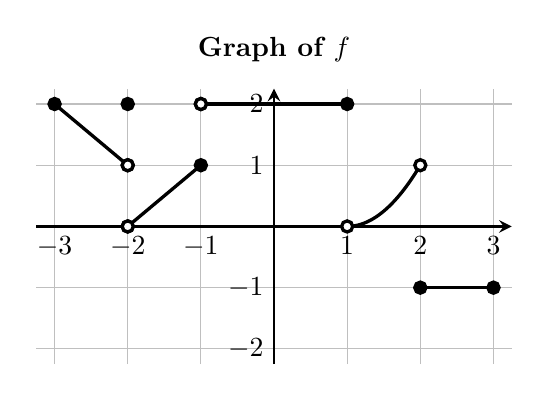
\begin{tikzpicture}
\begin{axis}[
   	xmin=-3.25, xmax=3.25,
	ymin=-2.25, ymax=2.25,
	major tick length={0},
	xtick={-3,-2,...,3}, ytick={-2,-1,...,2},
	line width=1pt, title={\textbf{Graph of $f$}},
 	axis lines=center, height=2 in, width=3 in, grid=major,
 	restrict y to domain=-2.25:2.25
	]
	\addplot [mark=*, black, smooth, very thick] plot coordinates {(-3,2)(-2,1)};
	\addplot [mark=*, black, smooth, very thick] plot coordinates {(-2,3)};
	\addplot [mark=*, black, smooth, very thick] plot coordinates {(-2,0)(-1,1)};
	\addplot [mark=*, black, smooth, very thick] plot coordinates {(-1,2)(1,2)};
	\addplot [mark=*, black, smooth, very thick] plot coordinates {(2,-1)(3,-1)};
    \addplot [black, smooth, very thick, samples=100, domain=1:2] {(x-1)^2};
    \addplot [black, only marks, very thick, mark=*, mark options={scale=1, fill=white}]
    coordinates{(1,0) (2,1) (-1,2) (-2,1) (-2,0)};
    \addplot [black, only marks, very thick, mark=*] coordinates{(-2,2)};
\end{axis}
\end{tikzpicture}
%\end{center}
}
\end{minipage}}

\newcommand{\ggraff}{
\begin{minipage}[l][.30\textwidth]{3 in}{
%\begin{center}
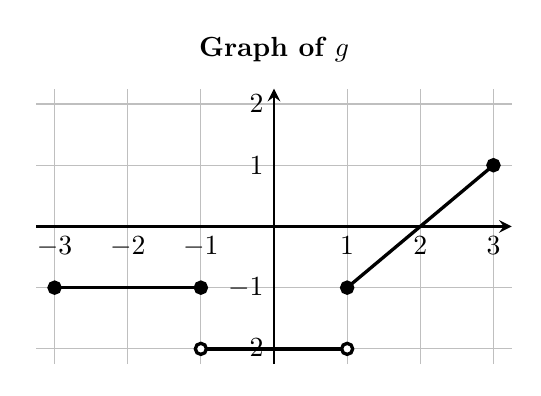
\begin{tikzpicture}
\begin{axis}[
   	xmin=-3.25, xmax=3.25,
	ymin=-2.25, ymax=2.25,
	major tick length={0},
	xtick={-3,-2,...,3}, ytick={-2,-1,...,2},
	line width=1pt, title={\textbf{Graph of $g$}},
 	axis lines=center, height=2 in, width=3 in, grid=major,
 	restrict y to domain=-2.25:2.25
	]
	\addplot [mark=*, black, smooth, very thick] plot coordinates {(-3,-1)(-1,-1)};
	\addplot [mark=*, black, smooth, very thick] plot coordinates {(1,-1)(3,1)};
	\addplot [black, very thick, mark=*, mark options={scale=1, fill=white}] plot coordinates {(-1,-2)(1,-2)};
\end{axis}
\end{tikzpicture}
%\end{center}
}
\end{minipage}}

\begin{document}
\begin{center}
    \large \textbf{Homework 1}
\end{center}
%\begin{itemize}
%    \item[\textbf{Week 1}]
            %\item Prerequisite Content:
                \begin{enumerate}
                    \item For each of the following, solve for the stated variable or expression.
                        \begin{enumerate}
                            \item $ \frac{x}{1-x}=b$; solve for $x$ in terms of $b$.
                            \item $ \left( \frac{x}{1-x}\right)\bigg/\left(\frac{p}{1-p}\right) = b$; solve for $x$ in terms of $p$ and $b$.
                            \item $ \left(\frac{x}{1-x}\right) \bigg/ \left(\frac{p}{1-p}\right) = \exp(b) = e^b$; solve for $x$ in terms of $p$ and $b$.
                            \item $ \exp(a)\exp(b)\exp(c)=\exp(x)$; solve for $x$ in terms of $a$, $b$, and $c$.
                            \item Suppose $ p_0 = \frac{\exp(a+bx)}{1+\exp(a+bx)}$ and suppose $ p_1=\frac{\exp(a+b(x+1))}{1+\exp(a+b(x+1))}$.  Write $ \left(\frac{p_1}{1-p_1}\right) \bigg/ \left(\frac{p_0}{1-p_0}\right)$ in terms of $a$, $b$, and $x$.
                            \item $ y_1-(mx_1+b)+y_2-(mx_2+b)+y_3-(mx_3+b)+y_4-(mx_4+b)+y_5-(mx_5+b)=0$; solve for $b$ in terms of the $x_i's$, $y_i's$, and $m$.
                        \end{enumerate}
                    \item Find the value of $c$ that makes the following identity hold. Your answer should depend only on $n$ and $p$ and not depend on $k$. \[\frac{(k-np)^2}{np}+\frac{((n-k)-n(1-p))^2}{n(1-p)}=\frac{(k-np)^2}{c}\]
                    \item Solve the following inequality for $n$ $$1-\left(\frac{\sigma}{t}\right)^2 \geq 0.99$$ when $t=0.05$ and $ \sigma = \frac{1.5}{\sqrt{n}}$.
                    \item Let $\sigma >0$ and $q >0$.  Consider the statement $ \frac{x-\mu}{\sigma} \in (-q, q)$, which is equivalent the the following inequality: $$-q < \frac{x-\mu}{\sigma} <q.$$  Find a value $a$ that depends on $\mu$, $\sigma$, and $q$, such that the inequality above implies that $x\in(-a,a)$. 
                    \item In statistics, the mean ($\mu$) of a set of numbers $\{x_1, x_2, \cdots, x_n\}$ is given by the formula $$\mu = \frac{1}{n}\sum_{k=1}^n x_k$$  Show that $$\frac{1}{n}\sum_{k=1}^n (x_k-\mu)^2 = \frac{1}{n}\sum_{k=1}^n x_k^2-\mu^2$$  FYI: The equation above demonstrates two expressions for variance, where the one on the right side is often considered an improvement for computational purposes.  You will use this improvement on the formula for variance in both the second foundations and the probability courses.
                    \item The following two equations will be encountered later in this course as part of a larger problem of finding maximum values of a multivariable function.  Solve each equation for the variable indicated. 
                       \begin{enumerate}
                           \item $ \frac{1}{\sigma^2}\sum_{k=1}^{n}(x_k-\mu)=0$; solve for $\mu$.
                           \item $ -\frac{n}{\sigma}+\frac{1}{\sigma^3}\sum_{k=1}^{n}(x_k-\mu)^2=0$; solve for $\sigma$.
                       \end{enumerate} 
                    \item Consider the function $ p(x) = \frac{1}{\sqrt{2\pi \sigma^2}}\exp\left( \frac{-(x-\mu)^2}{2\sigma^2}\right)$, which is the normal probability density function.  Let $h(x) = \ln(p(x))$.  Express $h(x)$ as a quadratic so it is of the form $ax^2+bx+c$. What are $a,b,$ and $c$? 
                    \item Suppose that $ f(i)= e^{-\lambda}\frac{\lambda^i}{(i+1)!}$.  Calculate $ \frac{f(i+1)}{f(i)}$, and fully simplify.
                    \item Say that $p(i)$ is defined below:
                        $$ p(i) = \begin{cases} 
                        c\cdot i & \text{if $1 
                        \leq i \leq 20, \quad i \in N$} \\
                        0 & \text{otherwise} \\
                        \end{cases}
                        $$
                        Find the value of the constant $c$ so that $ \sum_{i=1}^{20} p(i)$ = 1. Then, using that value of $c$, find $ \sum_{i=1}^{20} i\cdot p(i)$ and $ \sum_{i=1}^{20} i^2 \cdot p(i)$. 
                    \item Write each of the following expressions using summation notation.
                        \begin{enumerate}
                            \item $ \frac{1}{3}+\frac{1}{9}+\frac{1}{27}+\frac{1}{81} + \frac{1}{243}+ \frac{1}{729}$
                            \item $ \frac{5^2}{2!}+\frac{5^3}{3!}+\frac{5^4}{4!} + \cdots + \frac{5^{19}}{19!}$
                            \item $2^{i_1} + 2^{i_2} + \ldots 2^{i_k}$
                        \end{enumerate}
                \end{enumerate}
                
%\end{itemize}
\end{document}
